\chapter{因果结构}\label{chpt:causal}

Raychaudhuri 方程

\section{时空}


参考系要求时空至少在某一开域 $U$ 的时间定向性:

规定参考系矢量场指向未来

取号差 $+2$。取一 Lorentz 流形 $(M,\bm g)$ 及其切丛 $TM$。对某点 $p\in M$,若矢量 $\bm v$ 的模方 $\bm v \cdot \bm v$ 为正、负或零,那就分别称为\textbf{类空}、\textbf{类时}或\textbf{类光}矢量。所有类光矢量之集 $C_N$ 构成 $T_p M$ 的子集,称为\textbf{光锥}。

指向未来矢量所构成的子集 $\tilde F_p\subset T_p\R^{1,3}$ 称\textbf{指向未来部分},另一部分 $\tilde P_p$ 同理称\textbf{指向过去部分}。

任一事件 $p$ 的全体非零类时和类光矢量可分为此二大类,然而无论弯曲还是平直,一点的切空间当然不受影响,因此弯曲 Lorentz 流形中任一点的非零类时、类光矢量的集合也可类似地分为两大部分。

只孤立地讨论 Lorentz 流形一点 $p$ 固然可任意指定,但在讨论全时空时,物理上有理由期望这种指定在从一个时空点到另一时空点的过渡中是连续的。

当然,并非所有 Lorentz 流形都能做到这一点:
    \begin{eg}
        考虑用圆柱面 $S^1\times\R$ 表示时空,设度规这样给定:沿着任意 $S^1$ 一圈,其上光锥将均匀地旋转 $180^\circ$。这样便无法连续地指定$\tilde F$,因为若尝试按此指定,则一定存在某母线 $\R$ 上的 $\tilde F$ 有 $180^\circ$ 的突变。不妨认为这样的 Lorentz 流形没有物理意义。
    \end{eg}
\begin{definition}
    能连续地指定未来光锥的 Lorentz 流形叫\textbf{时间可定向的}(time orientable) Lorentz 流形。
\end{definition}
\begin{theorem}
    存在连续类时矢量场的 Lorentz 流形等价于时间可定向 Lorentz 流形。
\end{theorem}
\begin{proof}
    充分性上,设 Lorentz 流形存在一个连续的类时矢量场,就可把其在每点的值所在部分指定为指向未来部分,进而使得指定是连续的。必要性证明需要其它数学知识,且可见 Penrose(1972)。
\end{proof}


注意,谈到物理上合理的时空一般还要求时间可定向条件,并认为每一时空点都已作了这样的连续指定,也就是\textit{时间定向的(time oriented)},即只要可定向,那么已规定好了的就是时间定向的。不过考虑到有时玩具模型也会在称呼上用“时空”,因此 Lorentz 流形的定义不必太苛刻。若严苛一点就是:
    \begin{definition}
        \textbf{时空}通常强调是\textbf{时间定向时空},即已做时间定向的时间可定向 Lorentz 流形。
    \end{definition}
    类时矢量场结合度规可确定出光锥,因此时间定向又可用 $C_N$ 场表示。换句话说,每一点的(未来)光锥决定了时空结构(准确说是因果结构)。一点光锥称局部的,而光锥场就称整体的。因此大尺度宇观结构需要研究其上光锥场。

    有一个重要的例子:
    \begin{eg}
        \textbf{闵氏时空}是 $(\R^4,\upeta)$(记作 $\R^{3+1}$),其中 $\R^4$ 是指在 4 维实空间基础上,赋予了通常拓扑 $\mathcal T_u$ 和最大非怪异图册 $\{(O_\alpha,\psi_\alpha)\}$ 的光滑流形;$\upeta$ 称为\textbf{闵氏度规场},其定义是:$\R^4$ 的自然坐标系 $\{x^\mu\}$(这当然是 $\{(O_\alpha,\psi_\alpha)\}$ 中的一个图)在切丛里导出的坐标基底场,应使 $\upeta$ 场的分量在 $\R^4$ 上处处等于 $\eta_{\mu\nu}$,即
        \eq{
            \upeta=\eta_{\mu\nu}\d x^\mu\otimes\d x^\nu.
        }
    \end{eg}



    排除怪异图册是为排除那些在物理上不太可能的微分结构(如怪异 $\R^4$)。通常说的平直时空是指 $\R^{3+1}$。但“平直性”$\iff$ Riemann 内禀曲率张量为零张量,因此严格来说平直时空只要求配上 $\upeta$,无关于时空背景 $M$。

\begin{definition}
    \textbf{世界线}指 $(M,g)$ 上的曲线或路径\footnote{注意,虽然狭义相对性原理限制了我们只在惯性系讨论物理,但现代理论认为狭相的研究背景就是 $\R^{3+1}$,因此可用现代几何语言讨论非惯性运动(进而非惯性系),即任意世界线。在一般的时空上更是可以谈及,且结合广义协变性,甚至是任意坐标系。毕竟坐标是对物理定律描述的冗余,类似于规范不变(但不同)。}。
\end{definition}

下面研究所谓的类时世界线。指向未来的切矢总满足 $\dv*{t}\cdot\bm e_0<0$,其实亦即 $\text dx^0/\text d t>0$,我们一般默认类时世界线上参数是这样选择的(显然能使参数单调)。准确来说,还要规定参数是均匀的,即保持切矢模长。这种参数称为仿射参数。甚至可以保证切矢归一:设 $C: I \rightarrow M$ 是类空或类时线(类光线线长总为零,不必讨论),则线上任一点 $C(t')$ 的切矢 $\dv*{t'}$ 的模长是 $t'$ 的函数。任意指定线上一点 $C\left(t_0\right)$ 作为线长测量零点,则 $[t_0,t]$ 对应曲线段的线长 $L=\int_{t_0}^t\sqrt{|g(\partial_{t'},\partial_{t'})|}\mathrm{d} t^{\prime}$ 是关于 $t$ 的函数。$L$ 本身也可充当该线的参数,称为\textit{线长参数}。由 $\mathrm{d} L=\sqrt{|g(\partial_{t'},\partial_{t'})|}\mathrm{d} t^{\prime}$ 可知,线长参数给出的切矢有单位长。

\begin{definition}
    若一段类时线的切矢均指向未来,且其参数为线长参数,则称为\textbf{类时世界线}(或\textbf{指向未来类时线})。在物理上,它的像与某个质点历程中的全部事件之集等同。
\end{definition}
\begin{definition}
    一段类时世界线的线长称为该过程\textbf{所经历的固有时}。对 $\left[\xi_{0},\xi_{1}\right]$ 中的任意 $\xi$,考虑类时世界线 $\alpha$ 从 $\alpha\left(\xi_{0}\right)$ 到 $\alpha(\xi)$ 所经历的固有时
    \eq{\tau(\xi)=\int_{\xi_{0}}^{\xi} \sqrt{-g(\partial_\zeta,\partial_\zeta)} \mathrm{d} \zeta,}
    则 $\tau={\tau}(\xi)$ 总存在逆函数 $\xi=\xi(\tau)$,所以 $\alpha$ 可用 $\tau$ 来参数化。该参数正是类时世界线的线长参数,故又称\textbf{固有时参数}。
\end{definition}
观者(其世界线类时)所配备的标准钟的读数是固有时的物理性定义,无论零点如何,任意两读数的差总是等于此过程的线长。




\section{可定向性}

\section{因果线}

\section{因果条件}



\begin{figure}[h!]\centering
    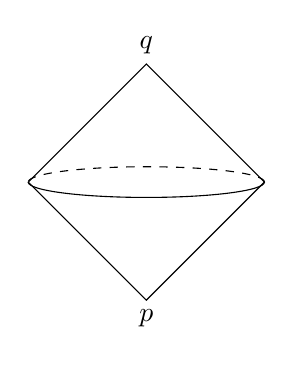
\begin{tikzpicture}[scale=1.5]
    \draw (0,1)node[above]{$q$}--(1,0)--(0,-1)node[below]{$p$}--(-1,0)--cycle;
    \draw[dashed] (1,0) arc [start angle=0, end angle=180, x radius=1, y radius=0.13];
    \draw (1,0) arc [start angle=0, end angle=-180, x radius=1, y radius=0.13];
    \end{tikzpicture}
    \caption{3 维平直时空的因果菱形。可见其形似一颗“钻石”,而其 2 维截面为“菱形”状(准确说呈平行四边形)。英语世界皆以“diamond”代之。}
\end{figure}

Cauchy 发展

\section{整体双曲时空}

渐近平直时空的共性变换
 
Raychaudhuri 方程

引力能量非定域性

\chapter{Cauchy 动力学与奇点定理}
\section{Witten 迅捷性}
\section{Penrose 过程}
\section{能量条件}
\section{奇点定理}
陷俘面
\section{宇宙监督假设}
\section{高-Wald 定理}


